% тут сейчас будут очевидные коментарии
\documentclass[12pt,a4paper]{article}
\usepackage[utf8]{inputenc}				% кодировка утф8
\usepackage[T2A]{fontenc}
\usepackage[russian]{babel}				% локализация
\usepackage{misccorr}					% пакет с дополнительными настройками для соответствия правилам отечественной полиграфии (не знаю, нужен ли, тупо скопипастил)
\usepackage{color}
\usepackage{graphicx}			% чтоб картинки вставлять
\usepackage{amsmath}					% для формул
\usepackage{amsfonts}
\usepackage{amssymb}
\usepackage{listings}                   % для вставок кода
\usepackage{hyperref}                   % оформление ссылок
\usepackage{blindtext}
%\usepackage[obeyspaces]{url}        % для путей и ссылок


\graphicspath{ {pic} }       % путь до картинок

%\color[named]{BrickRed}
%\pagecolor[named]{Green}

\begin{document}

\begin{titlepage}
\title{Разработка USB устройства ввода в Linux}
%\thanks{Version 1.0}
\author{Михаил Белкин}
\maketitle
\end{titlepage}

\tableofcontents
\newpage

\section{Схемотехника.}
\subsection{Выбор редактора.}
    Разработка схемы производится в KiCAD, это очень легковесный и компактный
    opensource редактор. Но при этом, несмотря на его внешнюю простоту, редактор
    как будто бы кричит нам "Я ничем не хуже чем этот ваш Altium и уж тем более
    Eagle". Поддерживается редактирование многослойных плат, так же используется
    профессиональный подход, при котором схема устройства и печатная плата
    редактируются отдельно. Так же он очень нетребователен к ресурсам
    компьютера.\\
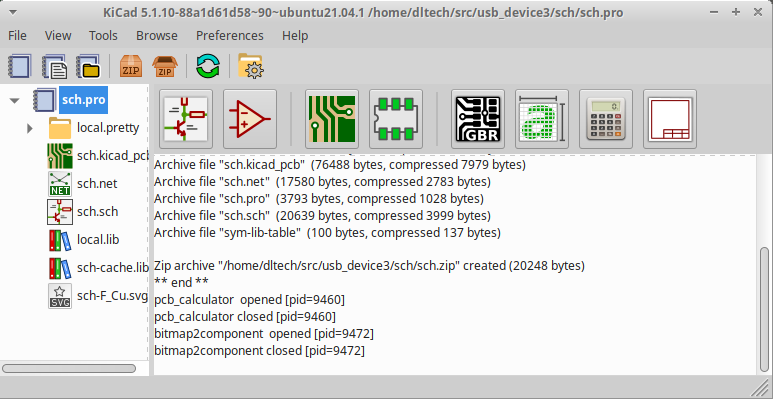
\includegraphics[width=10cm]{kicad1.png}\\
    К редактору имеется собственная библиотека компонентов, которая включает в
    себя компоненты всех популярных производителей. Но если вы принесли
    с китайского базара какую то экзотику, компонент придется разработать
    самостоятельно.\\
    Вывод шаблона печатной платы возможен во всех удобный форматах, включая pdf.
    Так же и Gerber и векторный svg, последнее очень удобно для печати шаблона
    на принтере. Единственное неудобство это не возможность сразу выводить схему
    в растровом формате, приходится самостоятельно конвертировать из svg.

\subsection{Установка редактора и библиотек.}
    Установка редактора в Ubuntu Linux производится очень просто, имеется
    отдельный ppa репозиторий с последней стабильной версией. В то время как
    наиболее полный набор библиотек компонентов можно скачать с гитхаба.\\
    Набор команд для установки KiCAD:
\lstset{language=bash}           % Задаем язык исходного кода
\begin{lstlisting}
sudo add-apt-repository --yes ppa:kicad/kicad-5.1-releases
sudo apt update
sudo apt install --install-recommends kicad
\end{lstlisting}
    Надеюсь устанавливать git вы умеете и про команду git clone вы тоже знаете.
    Вот ссылки на репозитории с библиотеками компонентов KiCAD:\\
    \url{https://github.com/KiCad/kicad-library}\\
    \url{https://github.com/KiCad/kicad-footprints}\\
    \url{https://github.com/KiCad/kicad-symbols}\\
    \url{https://github.com/KiCad/kicad-packages3D}\\
    Установив редактор и добавив библиотеки вы сможете открыть проект со схемой
    устройства
    \href{https://github.com/dltech/usb_device3/tree/main/sch}{по аресу}

\subsection{Выбор элементной базы.}
\subsubsection{Микроконтроллер}
    Для наиболее аккуратной реализации нужен современный микроконтроллер (МК) с
    полноценным аппаратным USB. Совершенно понятно, что таким микроконтроллером
    окажетcя STM32F103C8T6. Мощное ядро ARM Cortex-M3 с их фирменным вложенным
    контроллером прерываний (NVIC) позволит с легкостью справиться с любой
    задачей. А с такой простой как USB геймпад уж тем более. На борту имеется
    64 килобайта FLASH и 20 килобайт SRAM. И этого настолько много, что можно
    вовсе не думать об оптимизации. Теперь о стоимости, когда то я покупал такой
    за 60 рублей, сейчас цена приблизилась к 200, что по прежнему сравнимо по
    стоимости с остальными морально устаревшими микроконтроллерами. Так же в
    пользу данного микроконтроллера говорит наличие подробной
    документации. О том, почему именно F103, тут все просто, это самый дешевый
    МК с USB из тех что может предложить компания ST microelectronics.
\subsubsection{Стабилизатор}
    В шине USB, как известно, 5В, а номинальное напряжение питания МК 3.3В.
    Поэтому необходим понижающий стабилизатор напряжения. Я рассматривал три
    марки стабилизаторов. Они приведены в таблице ниже:
\begin{center}
  \begin{tabular}{ | l | l | l | l | l | }
    \hline
    стаб & $U_{in max}$ & корпус & производитель & особенности \\ \hline
    L78L33 & 30 & SOT-89 & ST microelectronics &  \\ \hline
    AMS1117-3.3 & 15 & SOT-223 & AMS semitech & термозащита \\ \hline
    XC6206-33 & 7 & SOT-23 & TOREX & CMOS \\ \hline
     \end{tabular}
\end{center}
    И если первый давно знаком многим радиолюбителям. То последние два это
    стабилизаторы от китайских производителей, которые появились недавно.
    В целом гораздо больше доверия к старому 78l, как минимум из за его
    большого входного напряжения. К тому же AMS1117 мне
    попадались нерабочими, и очень легко пробивались от скачков напряжения,
    не спасая нагрузку. Но хотелось бы компактней и подешевле, к тому же
    компьютер сам по себе стабильный источник питания. Поэтому я выбрал XC6206.
    Довольно необычный новодел на полевых транзисторах, в то время как другие
    два на биполярных. Ниже приведена его структурная схема, на которой видны
    еще и защитные антистатические стабилитроны.\\
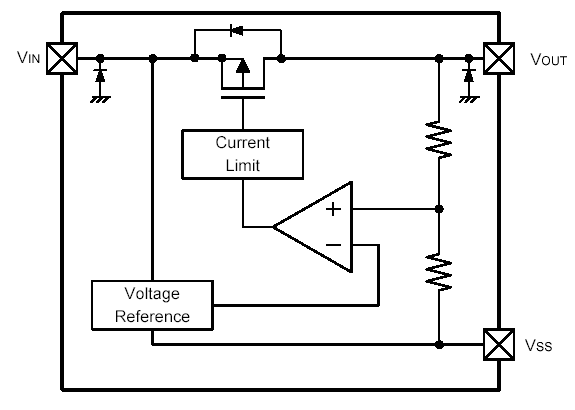
\includegraphics[width=10cm]{6206.png}
\subsubsection{Мелочь}
    На форумах можно услышать совет не ставить кварц в целях экономии. Но в
    в случае с асинхронной шиной кварц нужен для
    стабильной работы устройства. Микроконтроллер можно настроить на работу от
    самого распространенного кварца на 8мГц. Не удивительно, что на алиэкспресс
    сразу же нашелся не только планарный, но и очень компактный вариант.
    Размером как 1206 чип резистор. \\
    Резисторы размером 0402 я успел заказать заранее. А вот шунтирующие
    конденсаторы пришлось выпаивать с донорских плат, потому они не такие
    компактные, как хотелось бы (0805). \\
    Расчетный ток потребления десятки миллиампер, потому для стабилизации
    питания хватит и чип керамики, благо такая есть даже на 10 мкФ.
    На всякий случай установлю токоограничивающий резистор по питанию.
    Основная его цель обезопасить компьютер от случайного короткого замыкания.
    Хотя в дорогих флешках на его месте можно встретить чип предохранитель.
    Продолжу экономить и на разъемах, попросту ограничусь площадками под
    проводки.

\subsection{Особенность схемотехники USB.}
    На сайте можно скачать целый документ, посвященный вопросу распайки USB
    разъема. Основной вопрос заключается в возможности программного отключения
    устройства от ПК. Моё же устройство будет всегда включено, поэтому
    подтяжка линии DP к питанию будет постоянной, и осуществляться резистором,
    а не управляться транзистором и портом микроконтроллера.
    Также важно не забыть про защитные резисторы. Провод у меня используется
    готовый от клавиатуры, потому разъем на плате не нужен.

\subsection{Схема устройства.}
    А вот и схема целиком, как видите, все шины питания подключены и
    заземлены фильтрующими конденсаторами. Кварц с нагрузочными конденсаторами
    в наличии, так же подтянут к земле и порт сброса. Все как советует официальная документация.
    Кнопки джойстика, как видно, подключены к портам напрямую, т.к. внутри МК
    уже имеются резисторы подтяжки к 3.3В. Так же не обошлось и без так
    называемого ''грязного хака``, для упрощения трассировки платы один из
    портов ввода-вывода (28 вывод) использован как вывод земли. Но в этом нет ничего плохого,
    ведь порты после сброса находятся в состоянии с высоким входным
    сопротивлением.\\
    Так же на схеме вы можете увидеть и стандартный разъем SWD для прошивки
    и отладки ПО. Ровно как и подключенный на землю вывод BOOT0 означает
    запуск прошивки из основной flash памяти. \\
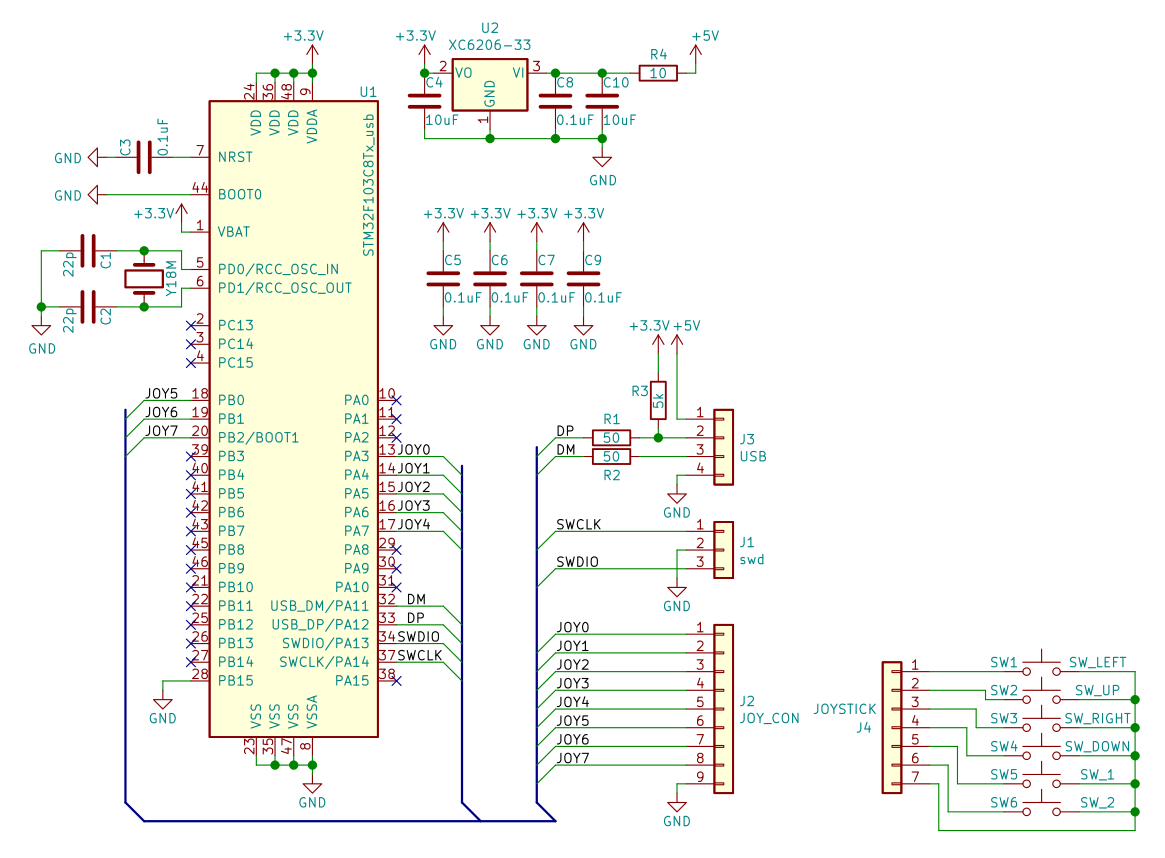
\includegraphics[width=15cm]{sch.png}\\

\newpage
\section{Программное обеспечение.}
    Если по началу, когда эти чипы только появились. Выбора способов написания
    ПО для них было немного. Как правило это были коммерческие среды
    среды программирования под Windows, которые студенты и любители как правило
    скачивали в месте с так называемой таблеткой от жадности. Теперь же выбор
    бесплатных инструментов очень большой. Начиная с официальной среды от
    компании ST, STM32Cube. Которая может не только скачать сама все их
    библиотеки и примеры, но и имеет автоматический конфигуратор периферии (это
    такая штука, которая предлагает настраивать регистры тыкая мышкой).
    И заканчивая сторонними продуктами, таким как AC6 system workbench.
    Так же на гитхабе полно примеров сборки через Makefile.
    А также комьюнити создало полноценную библиотеку libopencm3 с кучей
    примеров.\\
    Но исходя из того, что пример данного устройства довольно простой. Напишем
    весь код полностью самостоятельно.

\subsection{Тулчейн.}
    Когда то просто скачивание и установка gcc была поводом для отдельной статьи.
    Я же отмечу только то, что gcc признает контроллеры на ядре Cortex M3. И
    в ubuntu устанавливается вот такой вот командой:
\begin{lstlisting}
apt install gcc-arm-none-eabi libnewlib-arm-none-eabi gdb-multiarch
apt install build-essential
\end{lstlisting}
    А наши makefile и скрипты прошивки их будут их искать потом как
    arm-none-eabi-gcc, arm-none-eabi-objcopy и gdb-multiarch.
    В остальном даже флаги компиляции в случае с данными микроконтроллерами
    ничем особенно не отличаются.

\subsection{Что нового в CMSIS.}

\subsection{Компоновщик.}
    Устройство довольно простое, почему бы по новой не написать целиком все.
    Итак, не совсем целиком. Если игнорирование официальной библиотеки от
    производителя это уже немного глупо, то игнорировать библиотеки создателей
    процессора просто нельзя. Итак, выбран процессор с ядром ARM Cortex M3,
    значит и будем опираться на файл
    \path{CMSIS_5/blob/develop/Device/ARM/ARMCM3/Source/GCC/gcc_arm.ld}.


\subsection{Структура проекта.}

\subsection{Опрос кнопок.}

\subsection{Периферия USB.}

\subsection{Дескрипоры USB.}

\subsection{Стандартный протокол USB.}

\subsection{USB HID}

\subsection{Отладка.}

%\begin{thebibliography}{9}

%\bibitem{lamport94}
%  Leslie Lamport,
%  Addison Wesley, Massachusetts,
%  2nd edition,
%  1994.
%\end{thebibliography}

%\begin{list}
%    \item 78L33
%    \item AMS1117-3.3
%    \item XC6206-33
%\end{list}

\end{document}
